%================================================================================
%=============================== DOCUMENT SETUP =================================
%================================================================================

%\documentclass[lang=ngerman,inputenc=ansinew,fontsize=10pt]{ldvarticle}
\documentclass[lang=ngerman,inputenc=utf8,fontsize=10pt]{ldvarticle}
	%PACKAGES

		\usepackage{parskip}
		\usepackage{subfigure}
		\usepackage{ifthen}
		\usepackage{comment}
		\usepackage{color}	
		\usepackage{colortbl}
		\usepackage{soul}
		\usepackage{tikz}
		\usetikzlibrary{shapes,arrows}
		\usepackage{tabularx}
		\usepackage{todonotes}

		
		\definecolor{lightgray}{rgb}{0.75,0.75,0.75}

		
%================================================================================
%================================= TITLE PAGE ===================================
%================================================================================

\title{Projektplan Flying Circus}
\subtitle{Projektpraktikum Informationsverarbeitung}
\author{Tobias Eden, Lorenz Kenndoff, Adam Ivankay, Thomas Riethorst}

\date{\today}

\begin{document}

	\maketitle	
	\thispagestyle{empty}

\hrule

\section*{Motivation}

Das Projektpraktikum Informationsverarbeitung stellt als Hands-on-Projekt die Schnittstelle zwischen Theorie und Praxis dar, welche besonders für Ingenieure von großer Bedeutung ist.
Das Thema des autonomen Fluges, welches auch den Schritt in Richtung Forschung macht, bildet damit eine interessante Grundlage für eigene Ideen und Entwicklungen. 
Dabei werden die während dem Studium angeeigneten Fähigkeiten und Kenntnisse des Teams im Bereich Regelungstechnik und Programmierung erweitert und weiter verbessert. 
Ein wichtiger Aspekt ist auch der  Konkurrenzkampf mit dem anderen Team, da dieser sowohl das Interesse als auch die Motivation aufrecht erhält.   




\vspace*{1cm}
\hrule


\begin{figure}[!b]
\centering

\includegraphics[width=0.4\textwidth]{logo_kl.png}
\end{figure}

\newpage

%================================================================================
%================================= CONTENT ===================================
%================================================================================

\section{Beschreibung des Projekts}

\subsection*{Zielsetzung}
In dem dreimonatigen Projektpraktikum soll ein Luftschiff konstruiert werden, welches autonom einen vordefinierten Hindernis-Parcours abfliegt und an einer markierten Stelle ein Rettungspaket abwirft. Dazu müssen folgende Kriterien und Aufgaben eingehalten werden:

\begin{itemize}
\item Das Team hat während der Mission keinen Zugriff auf das Steuerungssystem des Luftschiffes 
\item Das Luftschiff soll ein Rettungspaket an einer zuvor definierten Position abwerfen
\item Das Luftschiff darf während der gesamten Mission nicht höher als 2m und tiefer als 0,5m fliegen
\item Die Dauer eines Durchlaufs zum Absolvieren der Mission beträgt maximal 15 Minuten, wobei zwei Durchgänge erlaubt sind
\item Sowohl die Gondel, als auch der Ballon dürfen Hindernisse im Raum nicht berühren
\end{itemize}

Bei der Entwicklung des Luftschiffes sind Umwelteinflüsse, wie Luftzug, IR-Störung, Helligkeits- und Temperaturänderungen zu beachten. Zusätzlich ist eine gewisse Toleranz in der Tragkraft des Zeppelinballons zu berücksichtigen.

\subsection*{Ansatz}
Unser Team hat sich für einen Ansatz mit drei Motoren entschieden, einen zur Höhenregelung und zwei für die Ausrichtung um die Gierachse. Das Grundgerüst der Gondel soll aus Carbonstangen gefertigt werden, woran der Ausleger für die Motoren befestigt wird. Verwendet wird ein IMU-Board zum Messen von Höhe, Luftdruck, Magnetfeld und Richtung; drei Motortreiber zur Steuerung und das Arduino-Board zur Berechnung der Steuerbefehle. Ein den Projektangaben entsprechendes Paket kann abgeworfen werden,  indem der haltende Draht kurzgeschlossen und somit durchgeschmolzen wird.


Das Gesamtkonzept sieht vor, die Wegfindung am PC zu berechnen. Die aktuellen Positionsdaten sowie die nächsten anzufliegenden Wegpunkte werden am PC berechnet und dann zum Arduino übertragen. Am Arduino wird dann durch die Regelsoftware die notwendige Kursänderung berechnet, die notwendig ist, um den nächsten Wegpunkt, ausgehend von der aktuellen Position, anzufliegen.


Für das Projekt stehen uns die Dokumentationen der letztjährigen Teams zur Verfügung, sowie das über die Jahre entwickelte Indoor-Positioning-System (IPS).


\newpage
\section{Projektumfang und Meilensteine}
Um eine zuverlässige Kontrolle des Projektfortschritts zu ermöglichen, sollen hier Meilensteine auf dem Weg zum vollendeten Luftschiff definiert werden, sowie die zum Erreichen dieser Meilensteine notwendigen Kriterien.

\begin{itemize}
	\item \textbf{Meilenstein Gondelhardware:} Datum: 13.05.2014
		\begin{itemize}
			\item Gondelskelett konstruiert
			\item Bauteile eingebaut und angeschlossen
		\end{itemize}
	\item \textbf{Meilenstein Funkverbindung:} Datum: 20.05.2014
		\begin{itemize}
			\item Funkverbindung Gondel - PC hergestellt
			\item Manueller gesteuerter Flug absolviert
		\end{itemize}
	\item \textbf{Meilenstein Höhenregelung:} Datum: 27.05.2014
		\begin{itemize}
			\item Funktionierende Höhenregelung
			\item Schwebeflug absolviert
		\end{itemize}
	\item \textbf{Meilenstein Autonomer Flug:} Datum 10.06.2014
		\begin{itemize}
			\item IPS einsatzbereit
			\item Wegfindungsalgorithmus erstellt
			\item Funktionierende Richtungsregelung
			\item Autonom gesteuerter Testflug absolviert
		\end{itemize}
\end{itemize}

\section{Projektstruktur}

\subsection*{Grundgerüst}
Das Grundgerüst dient der exakten Befestigung aller Komponenten der Gondel.\\
Als Aufbau unseres Grundgerüsts haben wir uns für einen Skelettaufbau aus Carbonstangen entschieden. Die Stift-/Buchsenleisten werden entsprechend mit den Carbonstangen per Epoxidklebstoff verklebt, um so ein stabiles und dennoch sehr leichtes Grundgerüst für die Gondel zu erhalten. Der Großteil der Elektronik kann somit einfach aufgesteckt und bei Bedarf getauscht werden, sollten Defekte auftreten. Die zwei Motoren zur Richtungsregelung werden an einem Ausleger aus Carbon fixiert.

Die Ultraschall-Sender für das IPS werden jeweils am Ende des Carbonauslegers montiert. Der Infrarotsender wird mittig positioniert. Der Motor zur Höhenregelung wird mittig auf einem kurzen Carbonausleger platziert. Sollten wir aus technischen Gründen (Ausgleich des Drehmoments bei nur einem Motor) auf zwei Motoren für die Höhenregelung umsteigen, werden diese auf dem großen Carbonausleger jeweils auf einer Seite montiert. Um die Trägheit um die Gierachse zu minimieren werden die schwersten Bauteile möglichst nah am Schwer-/Drehpunkt angebracht.
\subsection*{Motor und Motortreiber}
Das Team hat sich primär für einen Antrieb mit drei Motoren entschieden, zwei für die Bewegung in der Ebene, einen für die Höhenregelung. Ein späterer Umstieg auf eine Variante mit zwei Motoren für die Regelung wird offen gehalten. Zur Ansteuerung der Motoren werden insgesamt drei Motorentreiber benötigt. Wir werden kleine, leichte DC-Motoren verwenden, daher können wir einfache Treiber in Form von H-Brücken verwenden. Die Ansteuerung der Treiber wird direkt vom Arduino übernommen. Die Befestigung und Entfernung der Motoren zur Richtungsregelung zum Schwer-/Drehpunkt wird experimentell ermittelt. Dabei muss ein Kompromiss zwischen Leistungsbedarf für eine Drehung und der Problematik einer zu großen Empfindlichkeit durch großen Achsabstand gefunden werden. Bei den Propellern ist darauf zu achten, dass es sich um Typen mit unterschiedlichen Drehrichtungen handeln muss und diese an den Gleichstrommotoren befestigt werden können.
\subsection*{Sensoren}
Das IMU-Board wird, um möglichst störungsfreie Daten zu erhalten, auf der Oberseite des Ballons befestigt. Dadurch können wir die Einflüsse der Magnetfelder der Gleichstrommotoren so gering wie möglich halten. Welche Messdaten verwendet werden können, muss experimentell ermittelt werden. Im Grunde gilt, mit dem Konzept der zwei Ultraschall-Sender auf dem Ausleger lässt sich im Prinzip das IMU-Board einsparen, da es zwei Punkte der Gondel positioniert, und dadurch die Ausrichtung des Ballons auch bestimmt werden kann. Es wird trotzdem verwendet, um mehrere Daten für Höhe, Richtung und Beschleunigung zu erhalten. Des weiteren wird ein Ultraschallsensor zur Höhenmessung eingesetzt.
\subsection*{Funkverbindung}
Um eine Funkverbindung mit dem PC zu erhalten, wird ein XBEE-Modul verwendet. Über diese Kommunikationsverbindung werden dann die Koordinaten von der Basisstation an den Ballon übertragen. Für Tests können damit auch manuelle Steuerungen übernommen werden. Zusätzlich können vom Ballon verschiedene Statuswerte an den PC übertragen werden.
\subsection*{Abwurfmechanismus}
Als Abwurfmechanismus wird ein Transistor zum Durchbrennen eines Drahtes zum Lösen des Pakets verwendet. Die Dicke des Drahtes sowie der benötigte Strom zum Durchbrennen müssen experimentell ermittelt werden. Bei Erreichen der Koordinaten der Abwurfstelle wird die Software im Arduino einen Transistor ansteuern, der dann den dünnen Draht kurzschließt und ihn somit durchbrennt. Dadurch wird das Paket abgeworfen.
\subsection*{Stromversorgung}
Der Akku wird aus zwei Zellen in Serie mit jeweils 3,7V, also insgesamt 7,4V, bestehen. Die Motoren sowie die Ultraschallsender können mit dieser Spannung umgehen. Für die restliche Elektronik werden noch entsprechende Spannungswandler (Schaltregler) für die Spannungen 5V und 3,3V benötigt.
\subsection*{Erweiterung des IPS}
Das IPS soll in einem neuartigen Ansatz betrachtet werden. Da es bei den vorherigen Teams immer wieder zu den Problemen einer genauen Positionsbestimmung sowie Orientierungsbestimmung des Ballons gekommen ist, haben wir hier folgenden Ansatz gewählt.
Durch Erweiterung des IPS um die Funktion eines zweiten Senders, soll eine genauere Bestimmung der Position des Ballons ermöglicht werden. Es werden am Ballon zwei Ultraschallsender jeweils an einem Ende des Auslegers montiert. Diese werden dann abwechselnd, entsprechend den Intervallen des IPS, senden. Dadurch kann die Basisstation zwei Objekte lokalisieren. Die IPS-Software muss entsprechend angepasst werden, sodass die Signale beider Sender getrennt empfangen werden kann.

Durch diese Methode und den geometrischen Eigenschaften der Anordnung der Sender (Abstand zueinander, waagrechte Lage, usw.), erhoffen wir uns somit eine genauere Bestimmung der Position des Ballons. Auch soll es uns dadurch möglich sein, die Orientierung des Ballons berechnen zu können. Diese Werte können dann unterstützend, bzw. sogar ersetzend für das IMU-Board dienen.


Zusätzlich werden weitere IPS-Bodenstationen aufgebaut, um eine bessere Abdeckung zu erreichen. Auch die Neuentwicklung bzw. Verbesserung der Bodenstationen durch gerichtete Ultraschallsensoren wird im Zuge des Projekts getestet und validiert.


\subsection*{Software-Architektur}
Auf der Basisstation werden ankommende IPS-Messdaten gefiltert und ausgewertet sodass dem Luftschiff eine Position in einem globalen Koordinatensystem bezüglich der Basisstation zugeordnet werden kann.

Diese Position wird dann vom Wegfindungsalgorithmus verwendet um einen Kurs festzulegen. Sobald die Positionen des Luftschiffes sowie eines zunächst anzusteuernden Wegpunktes in das Koordinatensystem des Luftschiffes umgerechnet sind, werden diese per Funk an das Luftschiff übertragen.


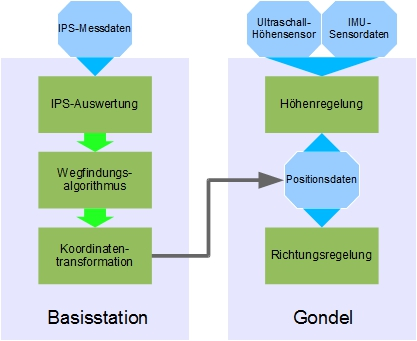
\includegraphics[scale=0.5]{Software}


Seitens des Luftschiffes kann nun die Regelung der Motoren aus den von der Basisstation gelieferten Daten sowie der Daten des IMU-Board und Ultraschallsensors stattfinden.

Der Befehl zum Abwurf des Pakets wird von der Basisstation ausgegeben sobald das Luftschiff die Abwurfzone erreicht hat.


\subsection*{Navigation und Wegfindung}
Aufbauend auf den Positionsdaten des IPS wird auf der Basisstation der optimale Weg durch den Hindernisparcours berechnet. Um Kollisionen mit den Hindernissen zu vermeiden wird ein Sicherheitsabstand um die Hindernisse festgelegt, welcher ungefähr dem doppelten Ballonradius entspricht. Die vollständige Flugroute des Luftschiffes im Slalom um die Hindernisse ergibt sich dann aus Kreissegmenten dieser Radien, welche tangential miteinander verbunden werden.


Der Wegfindungsalgorithmus wird bei Flugbegin zunächst einmalig ausgeführt und erzeugt Wegpunkte, welche der Gondel übermittelt werden und von der Regelungssoftware auf der Gondel weiter verarbeitet werden. Der Flug der Gondel wird laufend von der Basisstation auf Kursabweichungen überprüft. Für den Fall dass die Gondel das Ziel verfehlt und somit ein Toleranzwert für das Einhalten des vorgegebenen Kurses überschritten wird, wird der Wegfindungsalgorithmus erneut ausgeführt und die neuen Wegpunkte der Gondel übermittelt.


Zur Veranschaulichung der laufenden Prozesse der Navigationssoftware, der Position der Gondel sowie dem Zustand des IPS-Systems soll eine graphische Oberfläche verwendet werden. In der dargestellten Karte werden Hindernisse und spezielle Wegpunkte (z. B. Abwurfort, Ziel) per Eingabe festgelegt. Für Notfälle soll auch eine manuelle Steuerung in die Software integriert werden.
\subsection*{Regelung}
Alle zur Regelung notwendigen Berechnungen werden vom auf der Gondel installierten Arduino-Board übernommen. Es werden lediglich die aktuellen Positionsdaten und die Position des nächsten Wegpunktes an die Gondel übermittelt. Zur Vereinfachung der Berechnungen auf der Gondel werden die Koordinaten vorher auf der Basisstation von einem globalen Koordinatensystem mit festem Ursprung in der Bodenstation auf das lokale Koordinatensystem der Gondel, dessen Ursprung  im Luftschiff liegt, umgerechnet. Zur Höhenregelung wird ebenfalls das IPS verwendet. Sollten jedoch die Höhenmessdaten des IPS zu unzuverlässig sein, wird ein Ultraschallsensor verwendet, der die Höhe des Ballons ermittelt. Eine weitere Methode zur Höhenmessung bietet sich in der Luftdruckmessung des IMU-Boards, welche jedoch starken, zufälligen Schwankungen unterliegen kann.\\ Ein entsprechender Höhenregelungsalgorithmus wird direkt auf dem Arduino implementiert.


Bei der Erstellung der Regelung muss darauf geachtet werden, dass das Regelungssystem Umwelteinflüsse wie Zugluft, Druckänderung sowie das durch den einzelnen Höhenregelungsmotor auftretende Drehmoment ausgleichen kann. Weiterhin muss vor allem die Höhenregelung auf den Verlust von ca.1g Gewicht durch Abwurf des Paketes während des Fluges ausgelegt sein.





\section{Zeitplan}

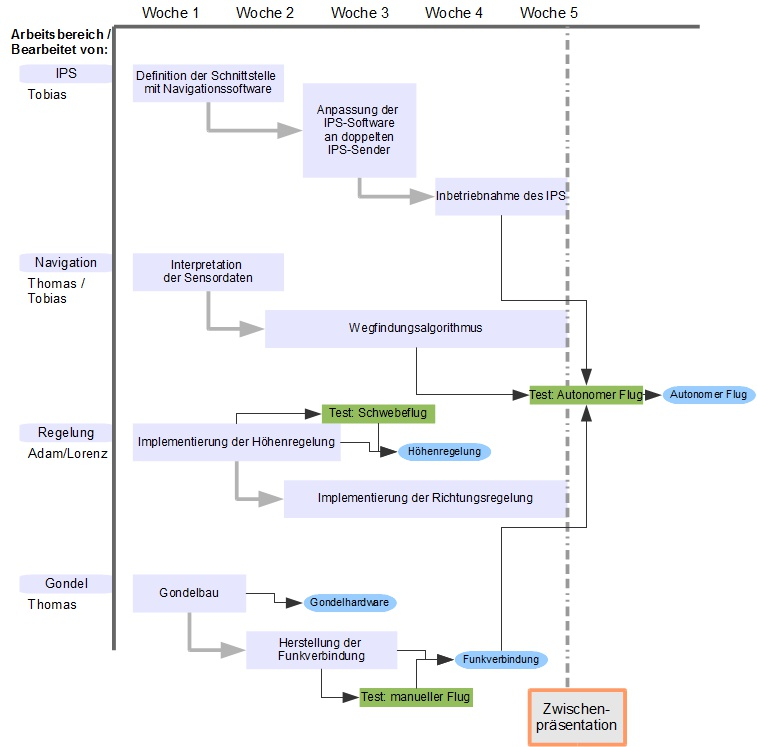
\includegraphics[scale=0.5]{Zeitplan-Arbeitspakete}


Wie die Grafik darstellt, wird in den ersten fünf Wochen ein Prototyp hergestellt, welcher bereits alle notwendigen Funktionen beinhaltet. Die oben definierten Meilensteine sind in blau hervorgehoben.


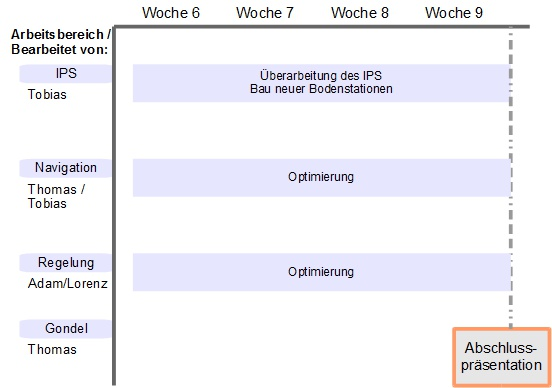
\includegraphics[scale=0.5]{Zeitplan-Arbeitspakete2}

\section{Material- und Kostenplanung}

Die im Bau der Gondel verwendete Hardware (vgl. Absatz „Aufbau des Grundgerüsts“) ist mit den folgenden Kosten verbunden:
\begin{tabbing}
Links \= Mitte \= Rechts \= rechtser \= rechtester \kill
Bauteil		\>\>\>\>		Kosten in Euro\\
==================================\\
Motoren:\>\>\>	\>			30\\
XBEE:	\>\>	\>\>		25\\
Motorentreiber:	\>\>\>\>	10\\
Propeller:		\>\>\>\>	5\\
Ultraschallsensor:\>\>\>\>  15\\
Spannungswandler:\>\>\>\>   5\\
Carbonstangen:	\>\>\>\>	5\\
Kleber:	\>\>	\>\>		vorhanden\\
Kabel/Lackdraht:\>\>\>\>	vorhanden\\
Arduino-Board:	\>\>\>\>	vorhanden\\
==================================\\
Summe:			\>\>\>\>	95\\
\end{tabbing}
Für die Motoren und Propeller sind hier bereits Ersatzteile im Preis einkalkuliert. Die XBEE Funkmodule werden gemeinsam mit dem anderen Team verwendet.

\section{Risikoanalyse}

Das wichtigste Abbruchkriterium ist das Überschreiten eines geplanten Zeitplans des Arbeitspakets. In dem Fall muss sich das ganze Team auf das Arbeitspaket konzentrieren und daran mitarbeiten. Da es im Team Personen gibt, die im Bereich Informationsverarbeitung Anfänger sind, ist eine realistische Planung vom Zeitaufwand der Arbeitspakete riskant, es müssen eventuell während des Projekts Änderungen vorgenommen werden. Die Evaluation der Meilensteine findet in gemeinsamen Treffen statt, jeweils direkt nach der Deadline des Arbeitspakets.


Ein weiteres Risiko besteht darin, dass die Resourcen nicht vorhanden sind, eventuell nicht zeitig geliefert werden können. Dies kann durch Umplanen und direktem Erscheinen in den Läden korrigiert werden. Der Beschädigung der einzelnen Bauteile soll durch sorgfältiges Einlesen und Informieren so gut wie möglich vorgebeugt werden.


Hinzu kommt noch, dass bei jedem Arbeitspaket Komplikationen auftreten können, wie z.B. Fehler bei der Programmierung, unvorhergesehene Störungen in der Hardware, konzeptionelle Fehler. In diesen Fällen muss das Team gemeinsam jeweils die bestmögliche Alternative finden (mögliche Risiken: Reichweite des IPS, Fehler im Code, Zwei Punkte-Positionierung des Ballons nicht genau genug, Umwelteinflüsse unberechenbar, Komplikationen mit der Wegberechnung, nicht richtig funktionierendes IPS).


Möglich, aber unwahrscheinlich ist, dass das vorgesehene Budget auf Grund von Beschädigung der Bauelemente nicht ausreicht; in dem Fall muss das Team mit dem Projektleiter konsultieren.

\section{Documentation}
Das Projekt wird während der Entwicklung laufend dokumentiert. Als Plattform für den Austausch von Dokumenten wird Github verwendet. Zum Abschluss des Praktikums wird ein umfassender Artikel zur Dokumentation unserer Ergebnisse auf dem Daedalus-Wiki veröffentlicht.

\section{Änderungen des Projektablaufes}
Alle auftretenden Änderungen dieses Projektplanes werden beispielsweise in einer Tabelle kurz notiert um Abweichungen und ggf. Änderungen des geplanten Ziels nachvollziehen zu können.



\begin{tabular}[htbp]{|p{0,025\textwidth}||p{0,06\textwidth}|p{0,4\textwidth}|p{0,37\textwidth}|}
	\hline
	\textsc{\#} & \textsc{Datum} & \textsc{Änderung} & \textsc{Grund} \\
	\hline
	\hline
	1 & & & \\[1em]
	\hline
	2 & & & \\[1em]
	\hline
	3 & & & \\[1em]
	\hline
	4 & & & \\[1em]
	\hline
	5 & & & \\[1em]
	\hline
	6 & & & \\[1em]
	\hline
	7 & & & \\[1em]
	\hline
	8 & & & \\[1em]
	\hline
\end{tabular}

\end{document}
